\documentclass{article}
%\usepackage{geometry}
%\geometry{top = 1in, bottom = 1in, left = 1in, right = 1in}
\usepackage[top = 0.7in, bottom = 0.7in, left = 0.7in, right = 0.7in]{geometry}
\usepackage{amsmath,amssymb,amsthm,mathrsfs}
\usepackage{graphicx}
\usepackage{bm}
\usepackage{float}
\usepackage[font=footnotesize,labelfont=bf]{caption}
\usepackage{movie15}
\usepackage{hyperref}

\usepackage{fancyhdr}
\pagestyle{fancy}
\rhead{\footnotesize {08/30/2012 ; MESA version 4411} }
\chead{\footnotesize {Authors: Jared Brooks, Lars Bildsten, Bill Paxton} }
\lhead{\footnotesize {mesa/star/test\_suite/he\_core\_flash} }

\begin{document}
	
	\begin{center}
	  \begin{Large}
	    \textbf{He CORE FLASH}\\
	  \end{Large}
	\end{center}

        This test is to show a 0.96 $M_\odot$ RGB star experiencing a helium core flash.  The run should be cut off when the log of the center temperature drops below 7.55 (\texttt{log\_center\_temp\_lower\_limit = 7.55}).\\

        The HR-diagram to the left (figure \ref{fig:1}) shows that surface conditions change relatively little during the core flash.  The plot to the right (figure \ref{fig:2}) shows that the core expands and cools.

        \begin{figure}[H]
          \begin{minipage}[b]{0.5\linewidth}
	    \centering
	    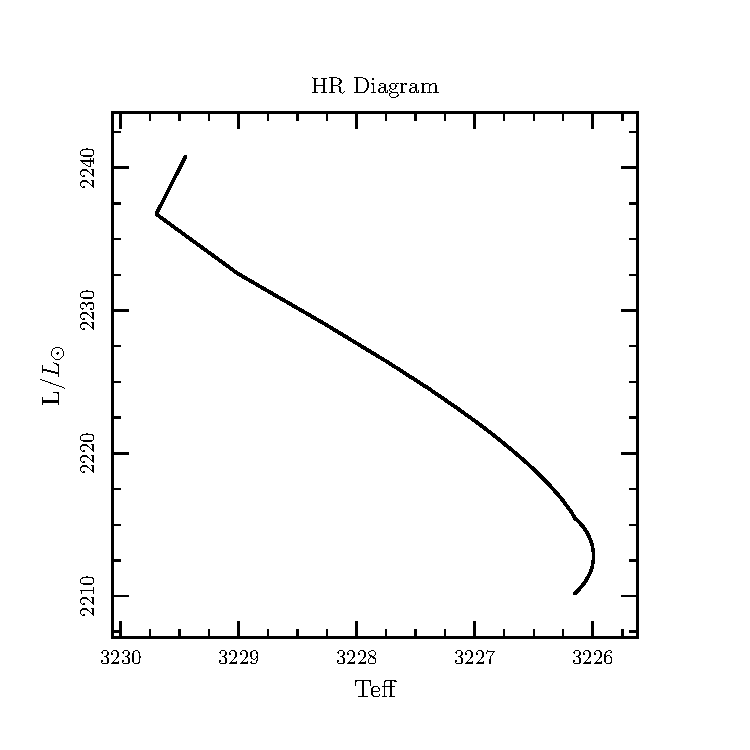
\includegraphics[width = 3.8in]{/Users/jaredbrooks/he_core_flash/plots_out/HR_Diagram.pdf}
	    \caption{HR-diagram shows surface changes relatively little}
	    \label{fig:1}
          \end{minipage}
          \hspace{0cm}
          \begin{minipage}[b]{0.5\linewidth}
            \centering
            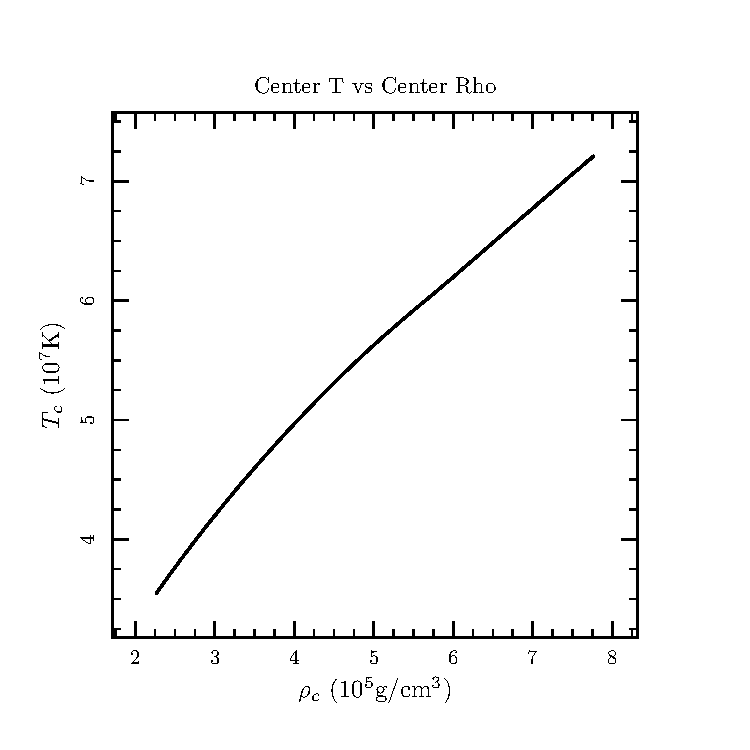
\includegraphics[width = 3.8in]{/Users/jaredbrooks/he_core_flash/plots_out/Tc_vs_Rhoc.pdf}
            \caption{The core expands and cools during the flash}
            \label{fig:2}
          \end{minipage}
	\end{figure}

        \pagebreak

        The plot to the left shows the evolution of the burning luminosities (figure \ref{fig:3}).  The elements in the core experience spikes in their burning luminosities during the flash, but the hydrogen burning outside the core experience a dip.  The plot to the right shows a profile of CNO burning rate and density against radius (figure \ref{fig:4}), with blue and black lines from before the flash, and light blue and grey from after the flash.  This shows that the core flash expanded, and thus cooled, the hydrogen burning shell and lowered the burning rate by almost six orders of magnitude.

        \begin{figure}[H]
          \begin{minipage}[b]{0.5\linewidth}
            \centering
            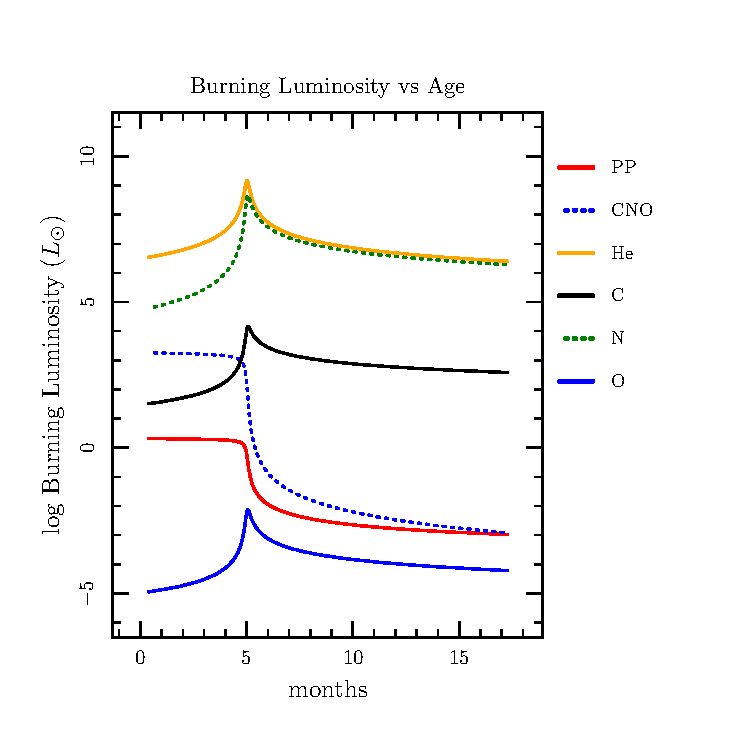
\includegraphics[width = 3.8in]{/Users/jaredbrooks/he_core_flash/plots_out/Burnrate_vs_Age.pdf}
            \caption{}
            \label{fig:3}
          \end{minipage}
          \hspace{0cm}
          \begin{minipage}[b]{0.5\linewidth}
            \centering
            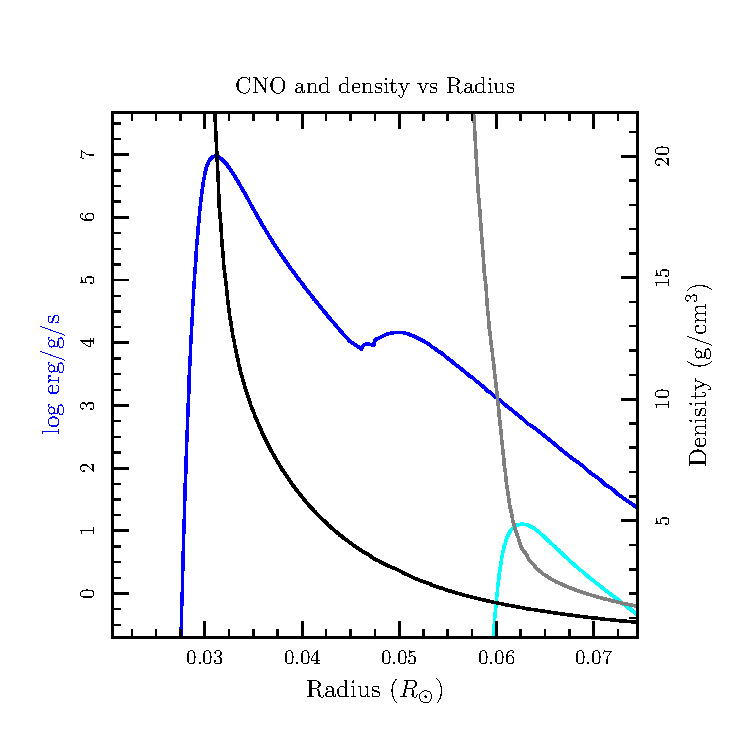
\includegraphics[width = 3.8in]{/Users/jaredbrooks/he_core_flash/plots_out/Burning_Rates_and_Density_vs_Radius.pdf}
            \caption{Blue=CNO before flash, Light Blue=CNO after flash, Black=Density before flash, Grey=Density after flash}
            \label{fig:4}
          \end{minipage}
        \end{figure}

        \pagebreak

        To the left is a burning rate profile from the peak of the flash (figure \ref{fig:5}).  To the right is an abundance profile from the end of the run (figure \ref{fig:6})

        \begin{figure}[H]
          \begin{minipage}[b]{0.5\linewidth}
            \centering
            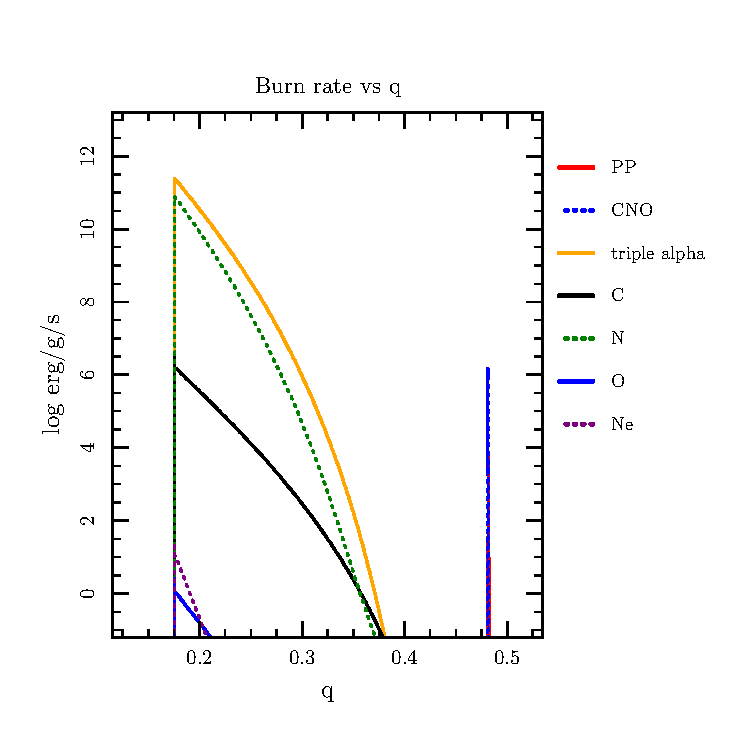
\includegraphics[width = 3.8in]{/Users/jaredbrooks/he_core_flash/plots_out/Burnrate_vs_q_9.pdf}
            \caption{Burning rate profile from peak of flash}
            \label{fig:5}
          \end{minipage}
          \hspace{0cm}
          \begin{minipage}[b]{0.5\linewidth}
            \centering
            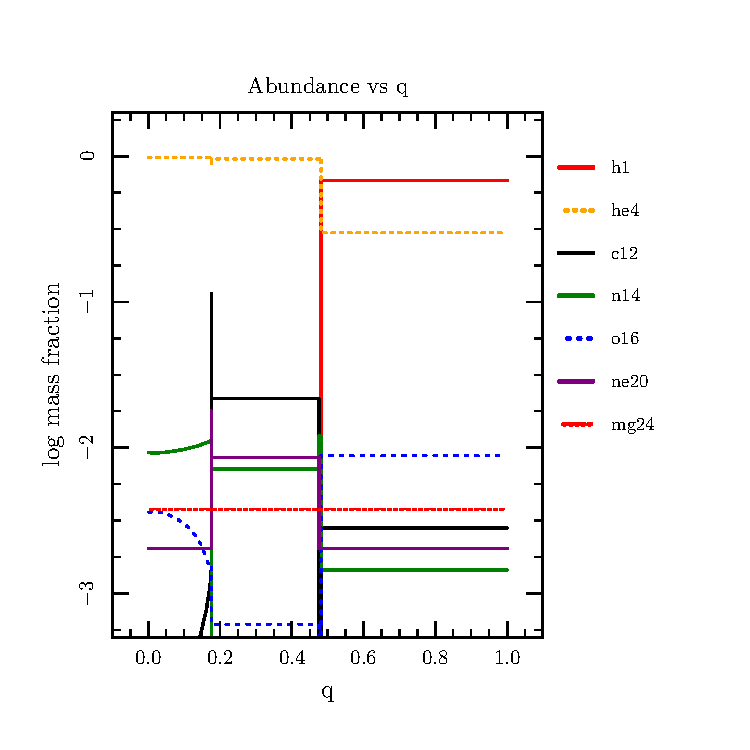
\includegraphics[width = 3.8in]{/Users/jaredbrooks/he_core_flash/plots_out/Abundance_vs_q_22.pdf}
            \caption{Abundance profile from end of run}
            \label{fig:6}
          \end{minipage}
        \end{figure}

        \pagebreak

        This final plot (figure \ref{fig:7}) shows a few internal \texttt{MESA} variables, such as the size of the time-step, the number of zones, and the number of retries against the model number in order to give some understanding of how hard \texttt{MESA} is working throughout the run and where some areas of problems/interest might be.

        \begin{figure}[H]
          \centering
          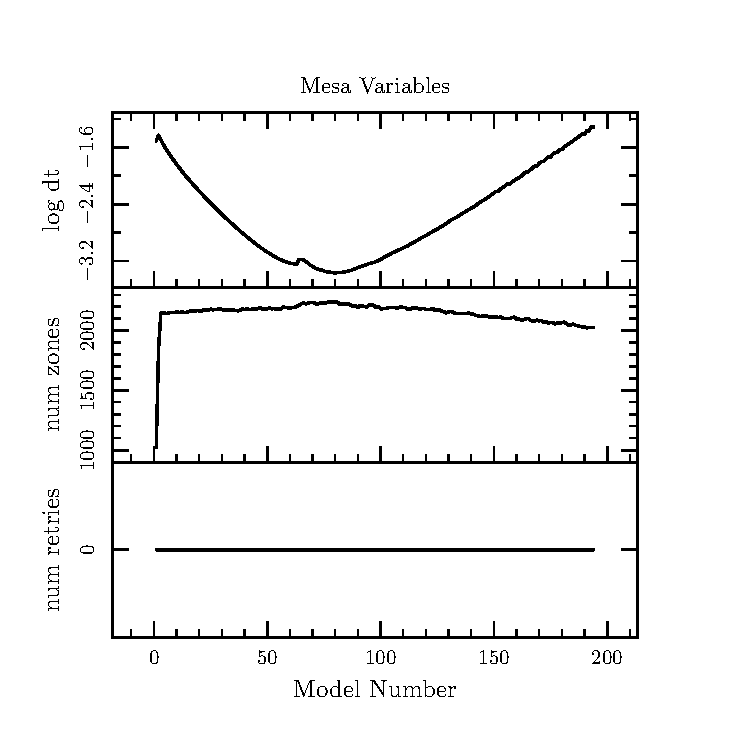
\includegraphics[width = 5in]{/Users/jaredbrooks/he_core_flash/plots_out/Mesa_Variables.pdf}
          \caption{\texttt{MESA} variables plotted against model number show how hard \texttt{MESA} is working}
          \label{fig:7}
        \end{figure}


\end{document}
